\section{Data}
\label{sec:data}

We confirm the behavior of the metrics on mock data with well-understood systematics as well as real data from past classification challenges.

\aim{Describe what mock data is: probability vectors}

\subsection{Mock classifier systematics}
\label{sec:mockdata}

\aim{Anita Bahmanyar will write the descriptions of and motivation for the confusion matrix-based systematics tests, as well as how the data is generated (what the underlying functions from the notebook are doing).}

For each, we will address:
\begin{enumerate}
  \item What defines this systematic?
  \item When has this systematic cropped up in the literature?
  \item What are our expectations for metric behavior?
\end{enumerate}

\subsubsection{Agnostic classifier}
\label{sec:agnostic_data}

uniform probabilities across all classes

\begin{figure}
	\begin{center}
		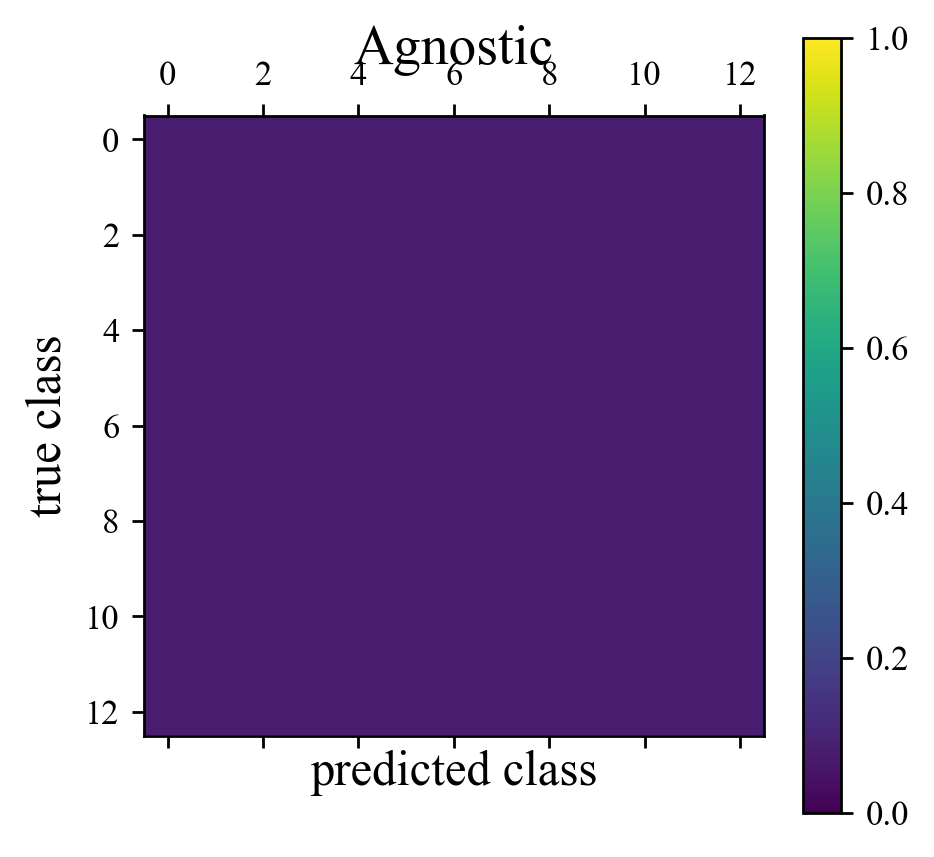
\includegraphics[width=0.45\textwidth]{./fig/Agnostic.png}\\
		\caption{}
		\label{fig:agnostic_data}
	\end{center}
\end{figure}

\subsubsection{Perfect classifier}
\label{sec:perfect_data}

perfectly accurate on all classes

\begin{figure}
	\begin{center}
		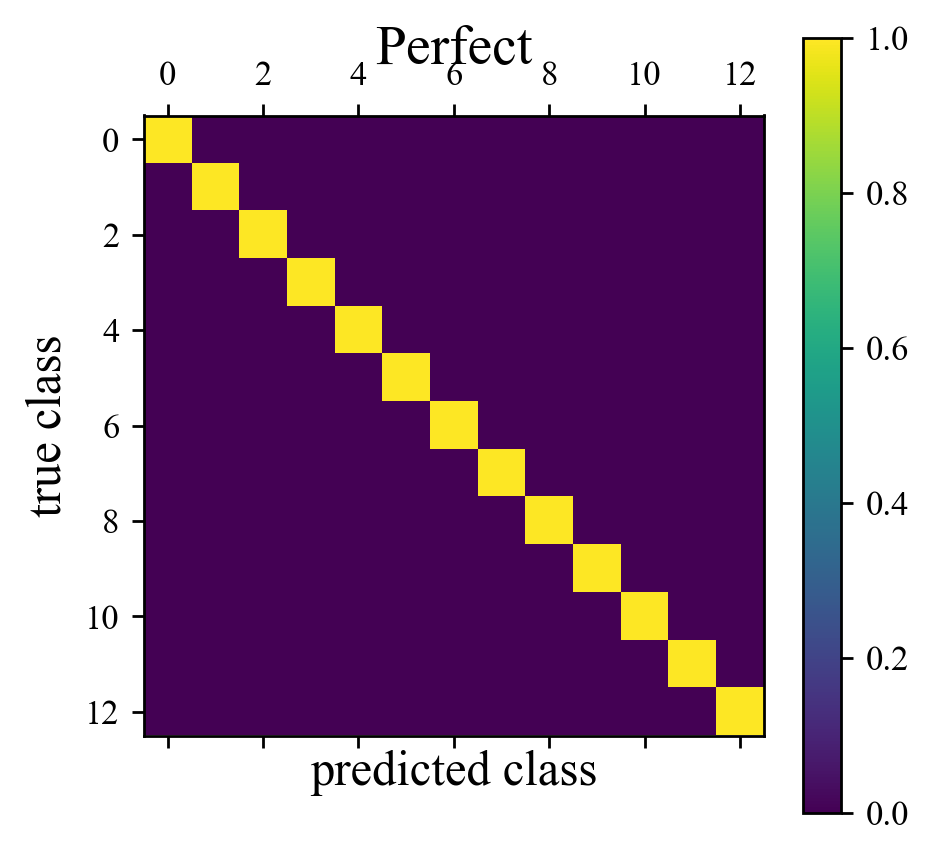
\includegraphics[width=0.45\textwidth]{./fig/Perfect.png}\\
		\caption{}
		\label{fig:perfect_data}
	\end{center}
\end{figure}

\subsubsection{Almost perfect classifier}
\label{sec:almost_data}

a slight perturbation of the perfect classifier

\begin{figure}
	\begin{center}
		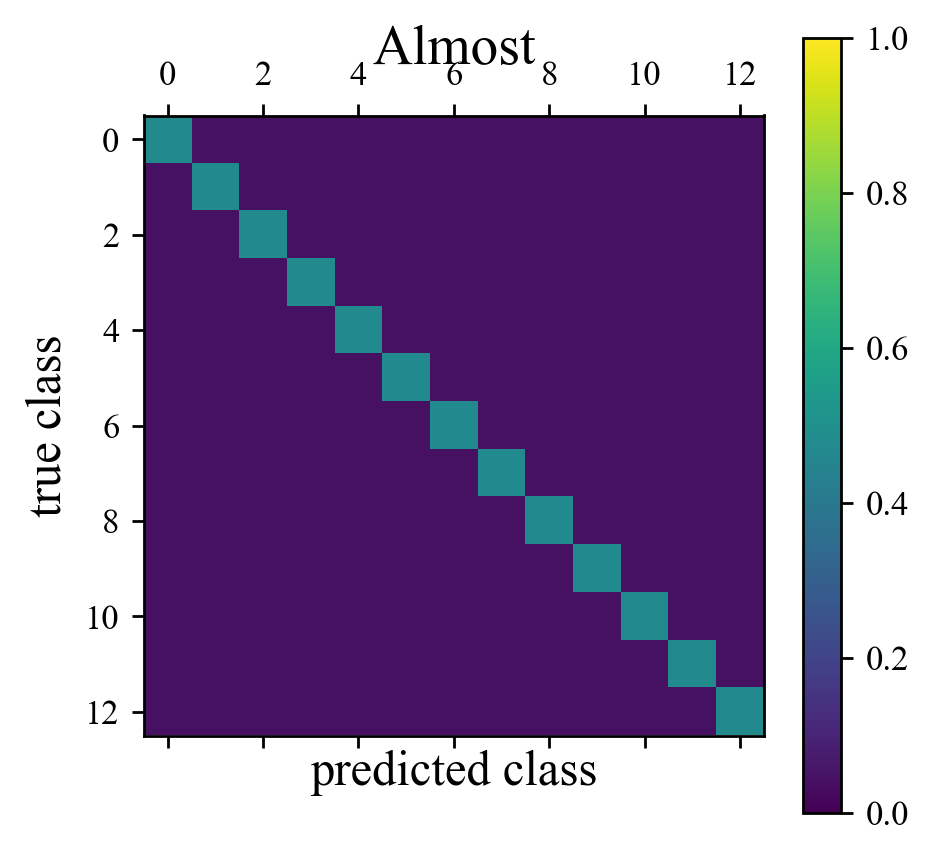
\includegraphics[width=0.45\textwidth]{./fig/Almost.png}\\
		\caption{}
		\label{fig:almost_data}
	\end{center}
\end{figure}

\subsubsection{Noisy classifier}
\label{sec:nois_datay}

a large perturbation of the perfect classifier

\begin{figure}
	\begin{center}
		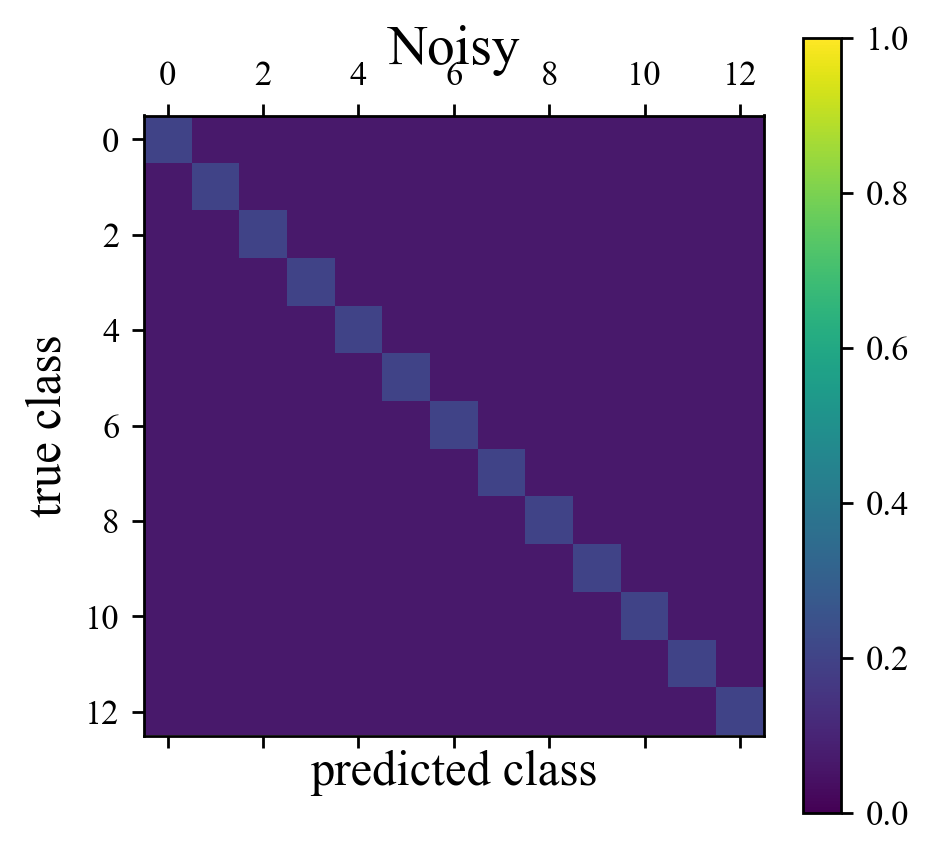
\includegraphics[width=0.45\textwidth]{./fig/Noisy.png}\\
		\caption{}
		\label{fig:noisy_data}
	\end{center}
\end{figure}

\subsubsection{Tunnel vision classifier}
\label{sec:tunnel_data}

classifies one class well and others randomly

\begin{figure}
	\begin{center}
		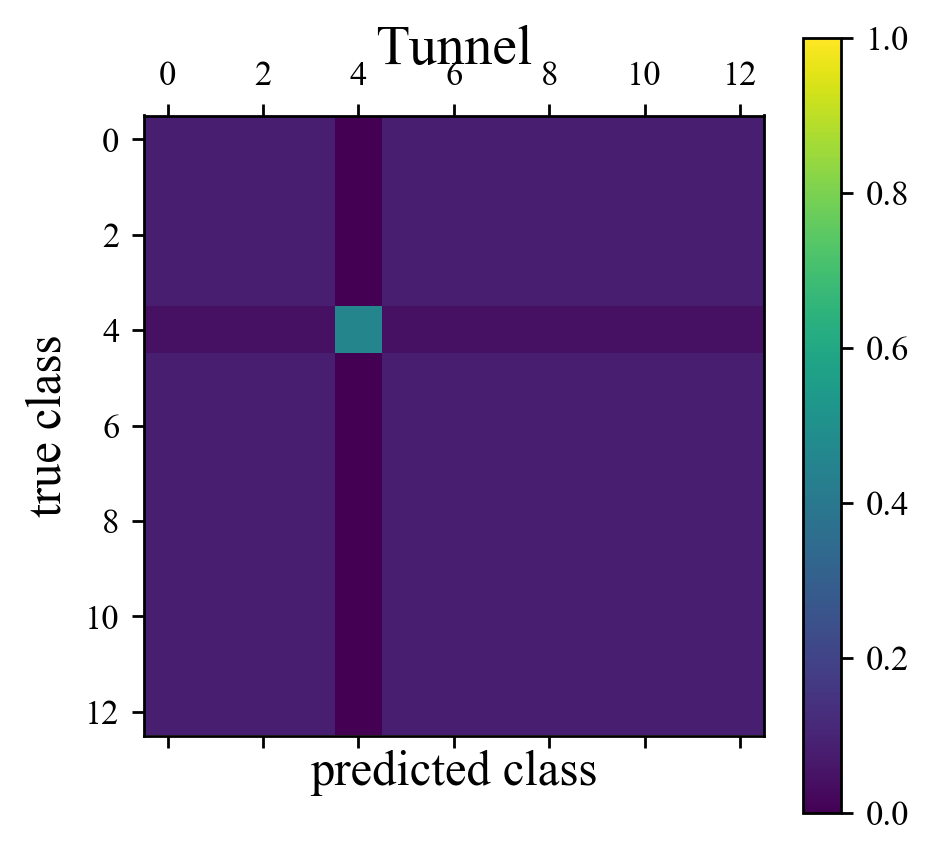
\includegraphics[width=0.45\textwidth]{./fig/Tunnel.png}\\
		\caption{}
		\label{fig:tunnel_data}
	\end{center}
\end{figure}

\subsubsection{Cruise control classifier}
\label{sec:cruise_data}

classifies all objects as a single class

\begin{figure}
	\begin{center}
		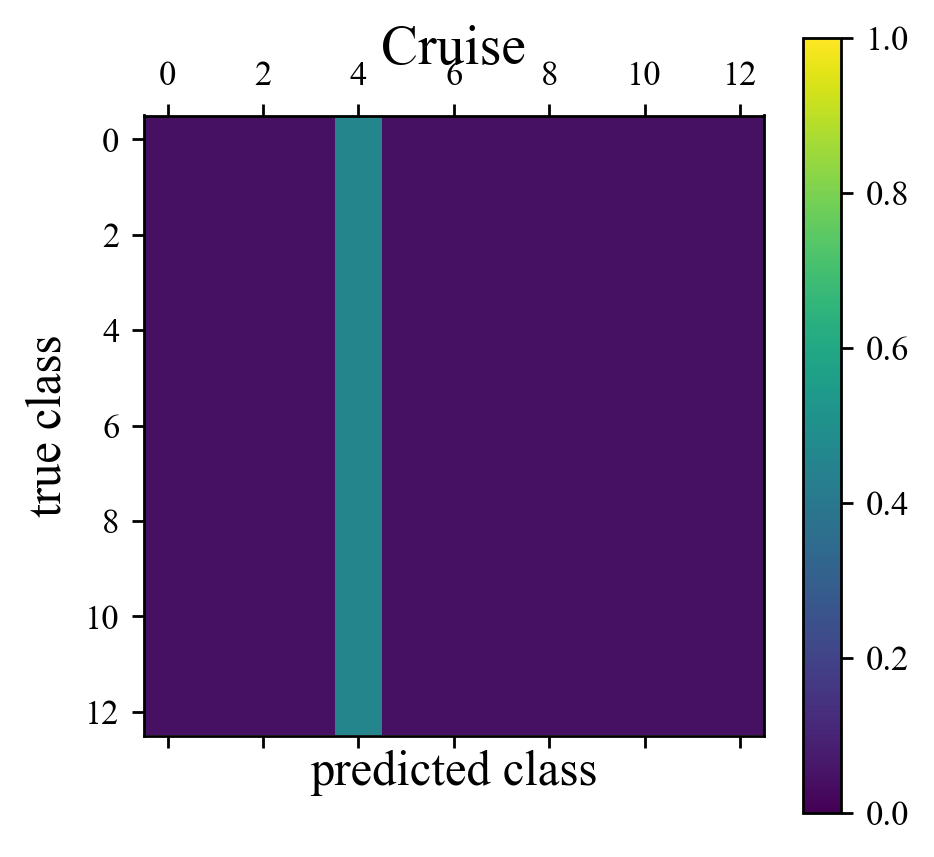
\includegraphics[width=0.45\textwidth]{./fig/Cruise.png}\\
		\caption{}
		\label{fig:cruise_data}
	\end{center}
\end{figure}

\subsubsection{Sumsuming classifier}
\label{sec:subsume_data}

consistently misclassifies one class as one other class

\begin{figure}
	\begin{center}
		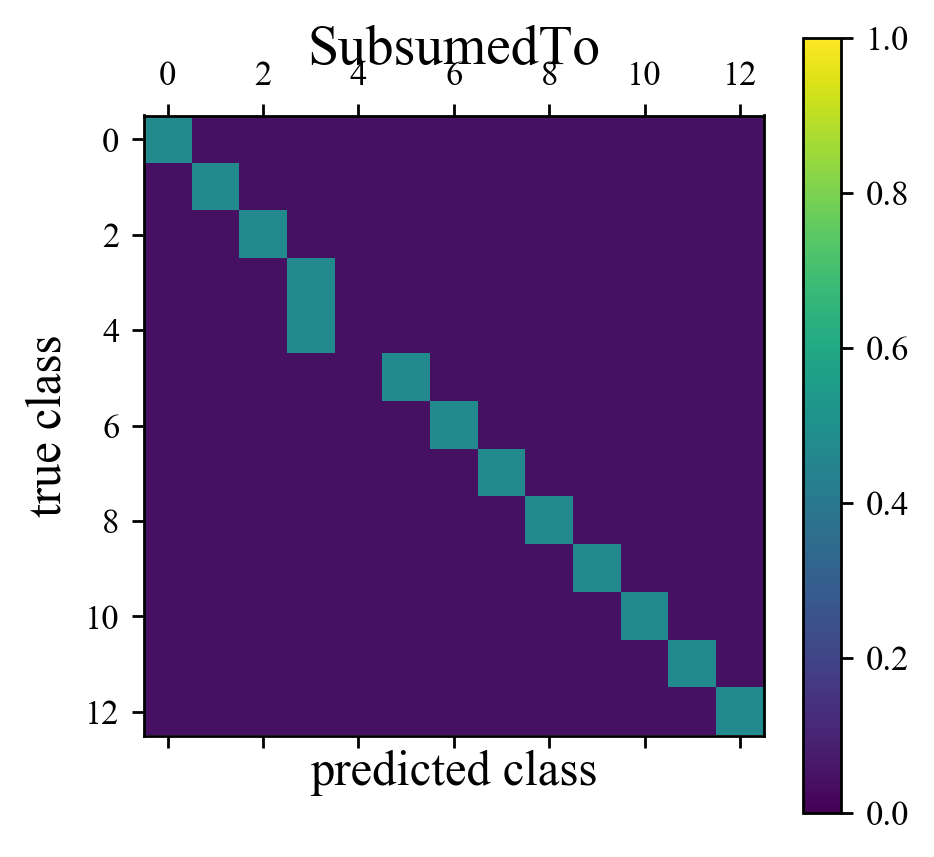
\includegraphics[width=0.45\textwidth]{./fig/SubsumedTo.png}\\
		\caption{}
		\label{fig:subsumer_data}
	\end{center}
\end{figure}

\begin{figure}
	\begin{center}
		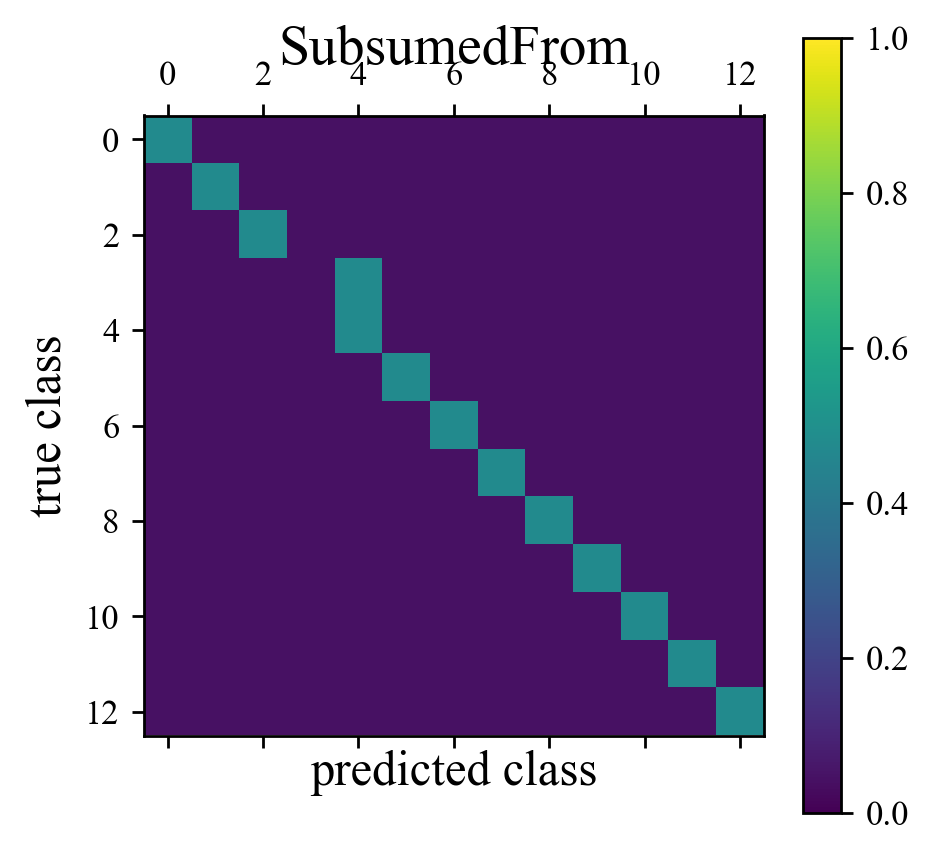
\includegraphics[width=0.45\textwidth]{./fig/SubsumedFrom.png}\\
		\caption{}
		\label{fig:subsumee_data}
	\end{center}
\end{figure}

\subsection{Representative classifications}
\label{sec:realdata}

\aim{Renee Hlozek will write the descriptions of these datasets.}

\subsubsection{SNPhotCC}
\label{sec:snphotcc}

\begin{figure*}
	\begin{center}
		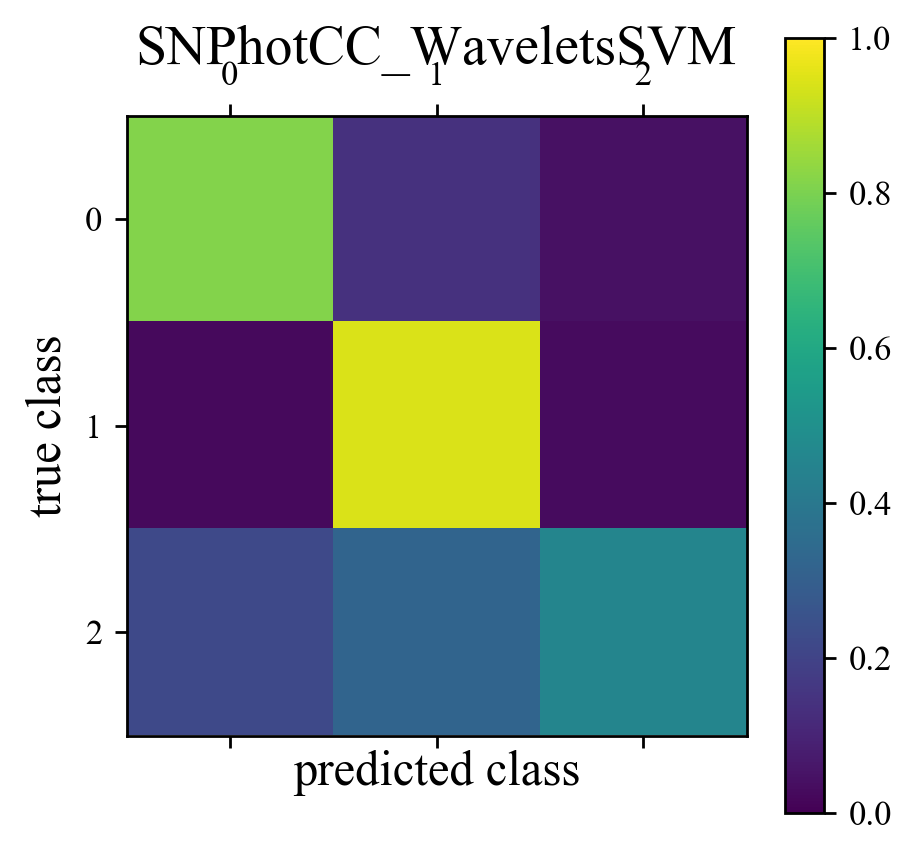
\includegraphics[width=0.24\textwidth]{./fig/SNPhotCC_WaveletsSVM_cm.png}
		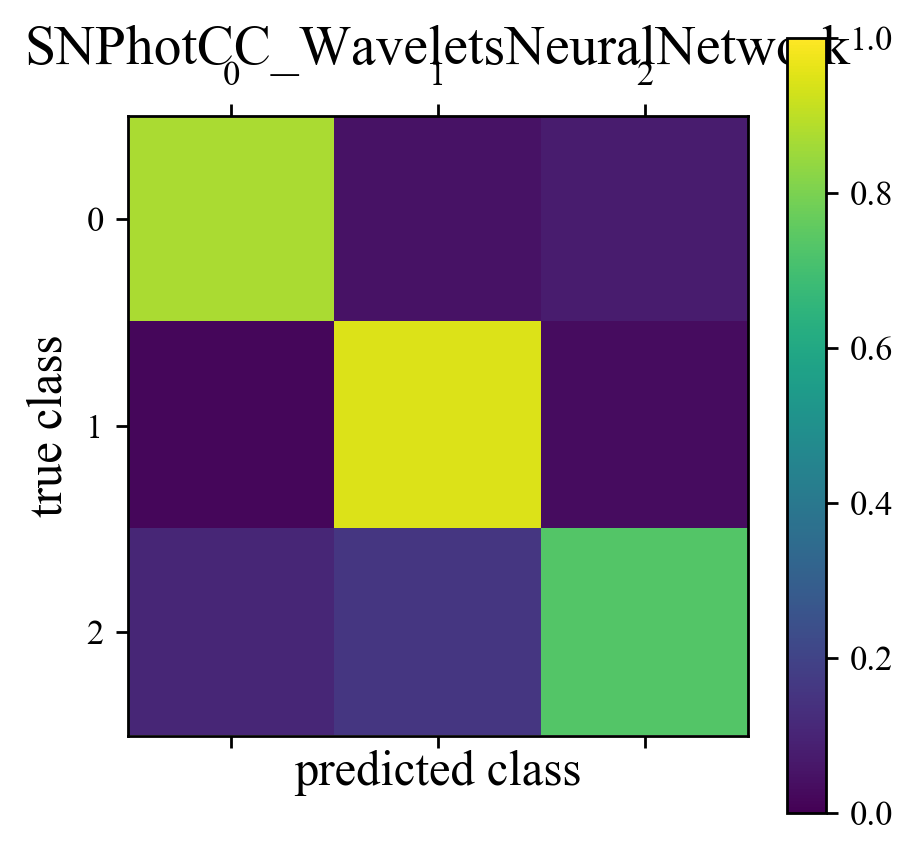
\includegraphics[width=0.24\textwidth]{./fig/SNPhotCC_WaveletsNeuralNetwork_cm.png}
		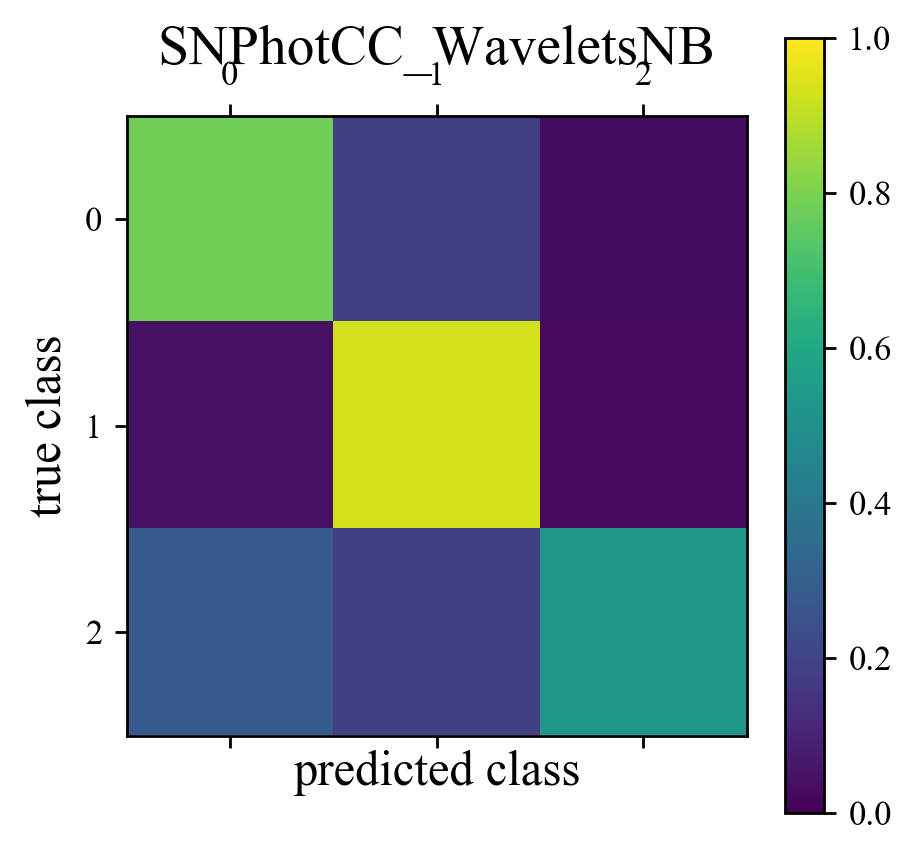
\includegraphics[width=0.24\textwidth]{./fig/SNPhotCC_WaveletsNB_cm.png}
		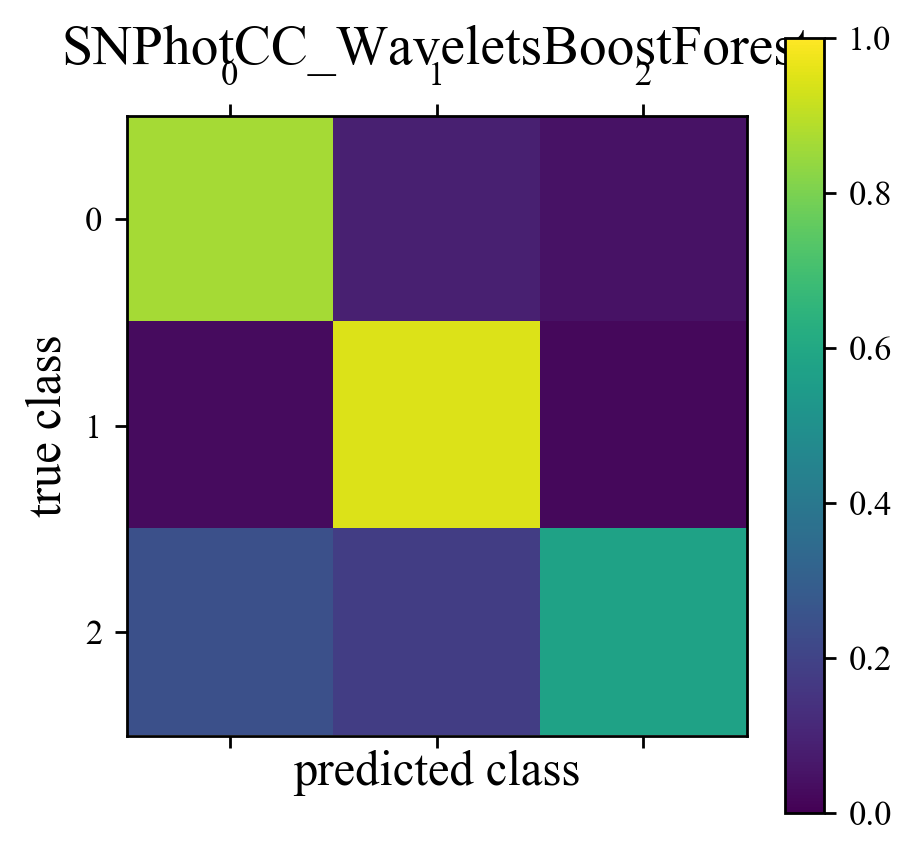
\includegraphics[width=0.24\textwidth]{./fig/SNPhotCC_WaveletsBoostForest_cm.png}\\
		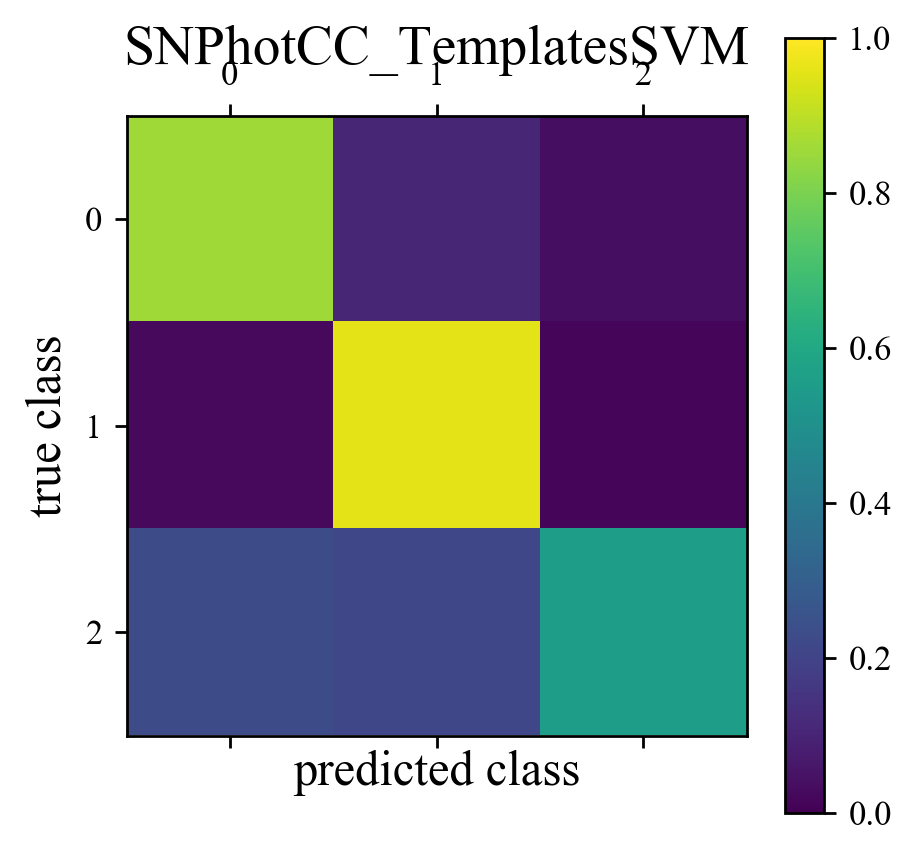
\includegraphics[width=0.24\textwidth]{./fig/SNPhotCC_TemplatesSVM_cm.png}
		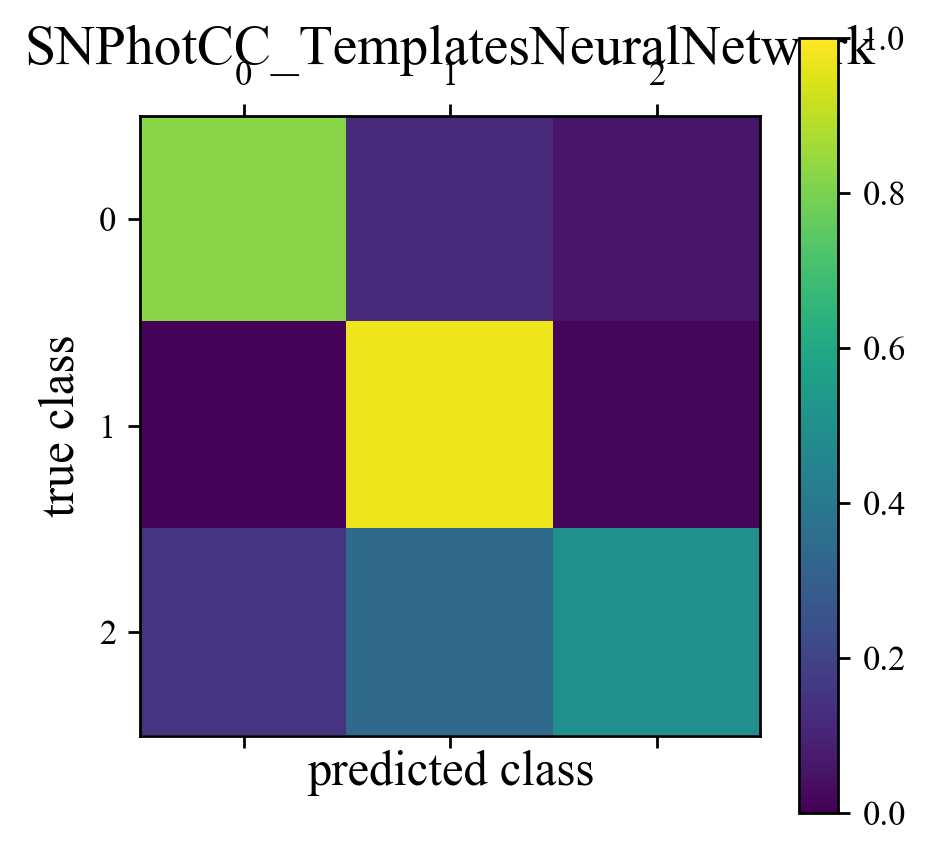
\includegraphics[width=0.24\textwidth]{./fig/SNPhotCC_TemplatesNeuralNetwork_cm.png}
		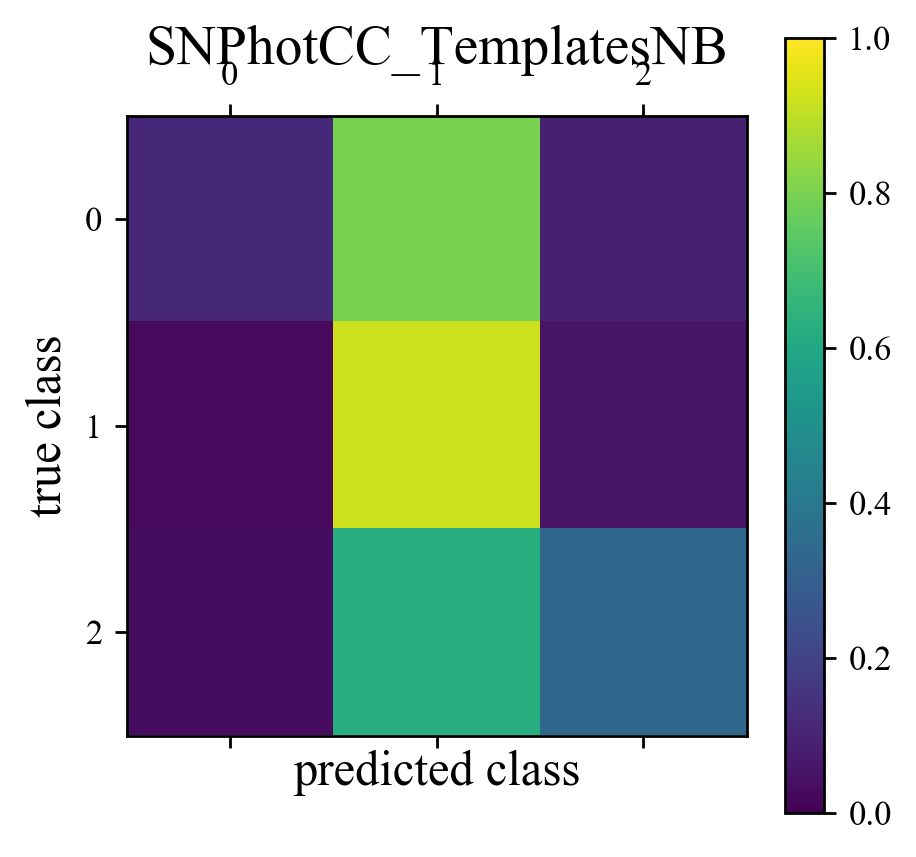
\includegraphics[width=0.24\textwidth]{./fig/SNPhotCC_TemplatesNB_cm.png}
		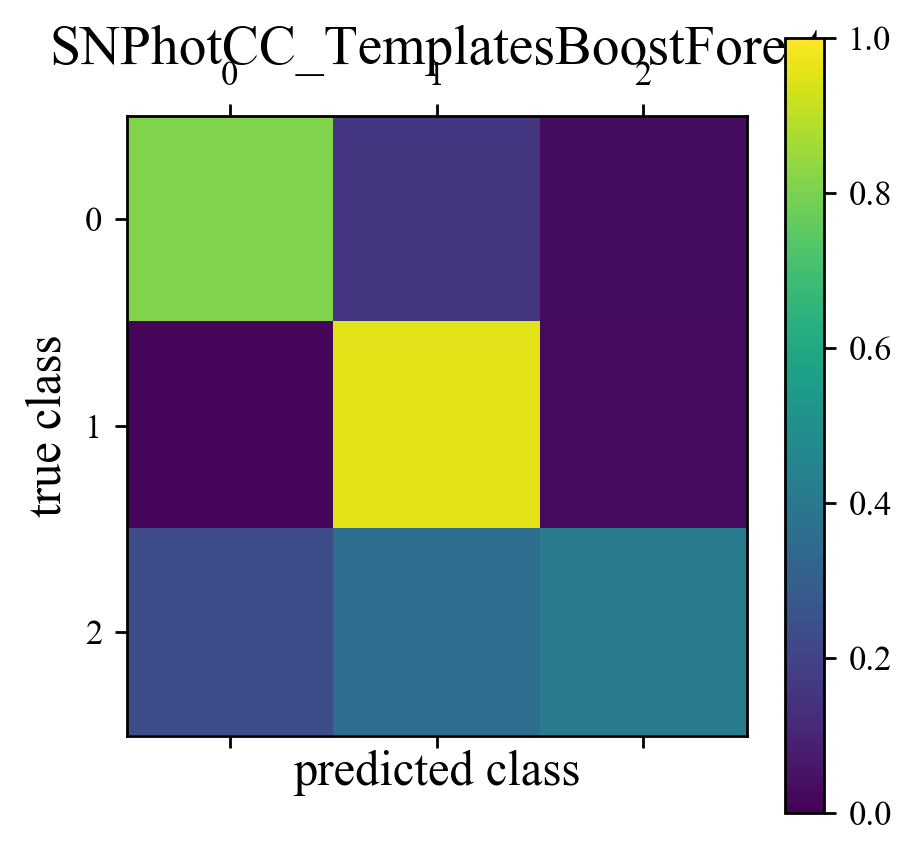
\includegraphics[width=0.24\textwidth]{./fig/SNPhotCC_TemplatesBoostForest_cm.png}
		\caption{}
		\label{fig:snphotcc_cm}
	\end{center}
\end{figure*}

\subsubsection{Unknown}
\label{sec:mystery}

\begin{figure*}
	\begin{center}
		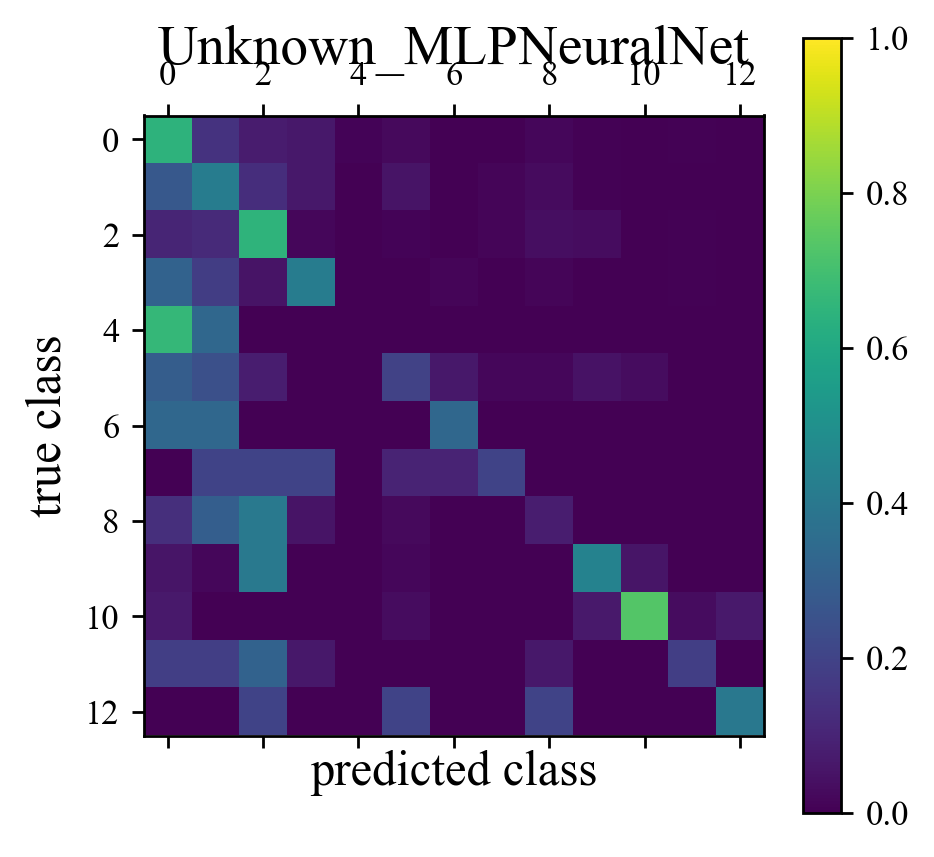
\includegraphics[width=0.3\textwidth]{./fig/Unknown_MLPNeuralNet_cm.png}
		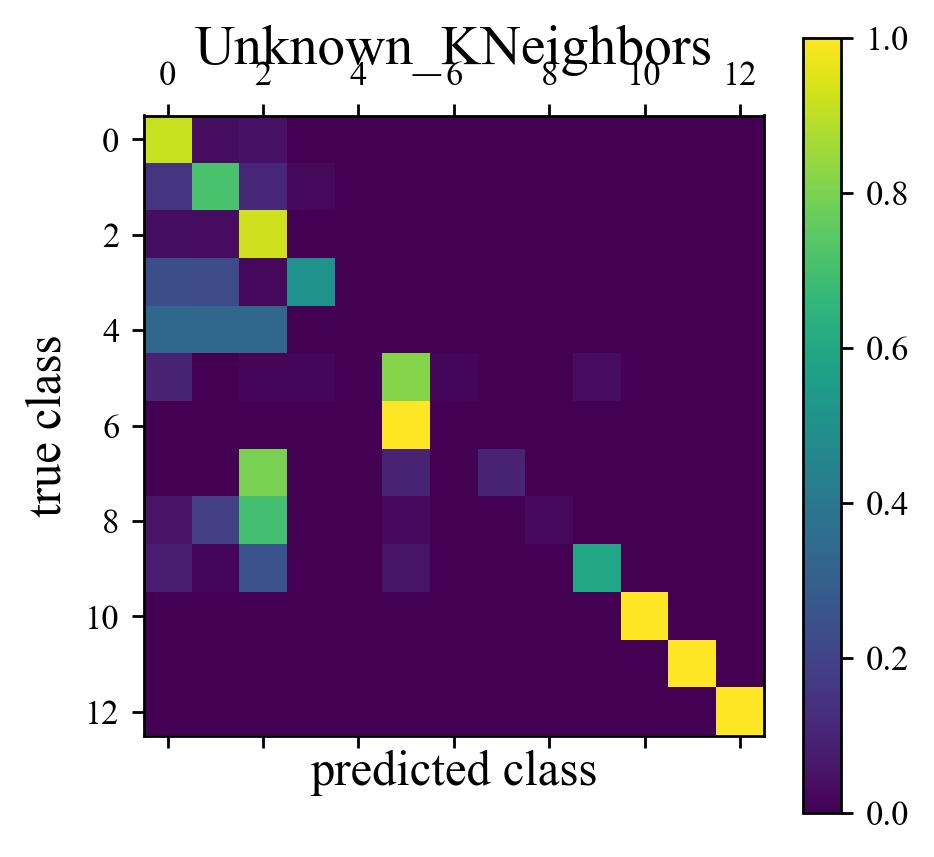
\includegraphics[width=0.3\textwidth]{./fig/Unknown_KNeighbors_cm.png}
		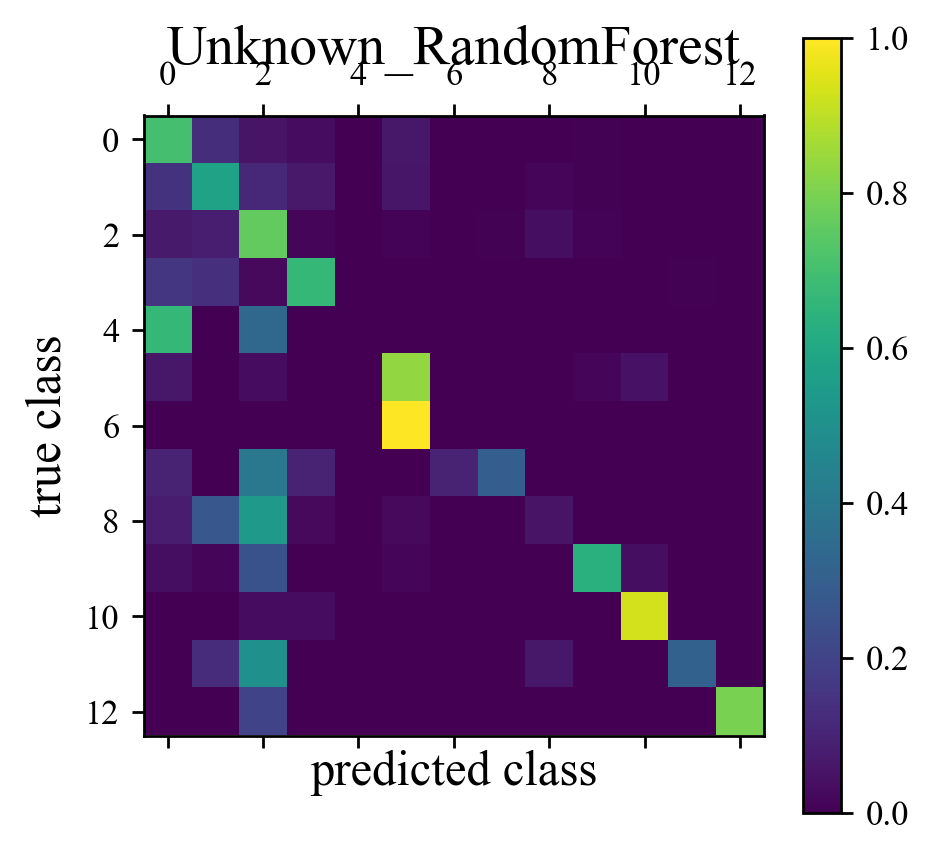
\includegraphics[width=0.3\textwidth]{./fig/Unknown_RandomForest_cm.png}
		\caption{}
		\label{fig:unknown_cm}
	\end{center}
\end{figure*}
